\documentclass[12pt,a4paper,oneside]{book}

% Packages
% Packages

% Language-related

\usepackage{setspace}
\usepackage[T1,T2A]{fontenc}
\usepackage[utf8]{inputenc}
\usepackage[english,bulgarian]{babel}

% Others
\usepackage{indentfirst}
\usepackage{amsmath}
\usepackage{blindtext} % Needed for creating dummy text passages
\usepackage[colorlinks=true,breaklinks,english]{hyperref}
\usepackage[hyphenbreaks]{breakurl}
\usepackage{xcolor}
\usepackage{ragged2e}
\definecolor{c1}{rgb}{0,0,0} % Blue
\definecolor{c2}{rgb}{0,0.3,0.9} % Light blue
\definecolor{c3}{rgb}{0.3,0,0.9} % Red blue
\hypersetup{
    linkcolor={c1}, % Internal links
    citecolor={c2}, % Citations
    urlcolor={c3} % External links/URLs
}

%\usepackage{cite} % Needed for cite

% Needed for cite and abbrvnat bibliography style
\usepackage[round,authoryear]{natbib}

% Needed for displaying bibliography and other in the table of contents
\usepackage[nottoc]{tocbibind}

\usepackage{graphicx} % Needed for \includegraphics
\usepackage{epstopdf}
\usepackage{longtable} % Needed for long tables over pages
\usepackage{bigstrut} % Needed for the command \bigstrut
\usepackage{enumerate} % Needed for some options in enumerate
\usepackage{todonotes} % Needed for todos
\usepackage{makeidx} % Needed for creating an index
\makeindex


% Page settings
% Page settings

% Needed for page border settings
\usepackage[top=1.8cm, bottom=1.8cm,left=2.0cm,right=2.0cm]{geometry}

% For writing with hyphenless justification (tries to)
\sloppy

\hyphenation{}
\hyphenpenalty=10000
\exhyphenpenalty=10000


% Custom commands

% This file defines some macros

% Text-bold-italic (makes the text bold and italic)
\newcommand{\tbi}[1]{\textbf{\textit{#1}}}

% Underline and italic
\newcommand{\imp}[1]{\underline{\textit{#1}}}


\begin{document}

\pagestyle{empty}
\begin{titlepage}

\center % Center everything on the page

\vspace{5mm}
\textsc{\Large Технологично училище Електронни системи към Технически
  университет - София}\\[0.5cm] % TUES ftw

\vspace{30mm}

{\Large \bfseries ДИПЛОМНА РАБОТА}\\[2cm]

\Large Тема: Мрежов анализатор с възможност за отдалечен анализ посредством
AngularJS 2 клиент

\vspace{40mm}

\begin{minipage}{0.35\textwidth}
\begin{flushright} \normalsize
Дипломант: \\[5mm]
Научен ръководител: \\[5mm]
\end{flushright}
\end{minipage}
~
\begin{minipage}{0.55\textwidth}
\begin{flushleft} \normalsize
Ивайло Арнаудов \\[5mm]
Стоил Стоилов\\[5mm]
\end{flushleft}
\end{minipage}\\[2cm]

{\normalsize София, $2017$} \\[0cm]


\vfill % Fill the rest of the page with whitespace

% List of symbols (kept just in case so far)

\newpage
\begin{flushleft}
\begin{Large}
\emph{\bf Списък на означения}\\
\end{Large}
\end{flushleft}
\begin{spacing}{1.241}
\vspace{10mm}
\begin{minipage}{0.2\textwidth}
\begin{flushleft} \normalsize
\ensuremath{\sigma_{y}(\tau)}\\
\end{flushleft}
\end{minipage}
~
\begin{minipage}{0.5\textwidth}
\begin{flushleft} \normalsize
Exponential regression function\\
\end{flushleft}
\end{minipage}\\[4cm]
\end{spacing}
\vfill

% List of abbreviations

\newpage
\begin{flushleft}
\begin{Large}
\emph{\bf Списък на съкращения}\\
\end{Large}
\end{flushleft}
\begin{spacing}{1.241}
\vspace{10mm}
\begin{minipage}{0.2\textwidth}
\begin{flushleft} \normalsize
VPN\\
\end{flushleft}
\end{minipage}
~
\begin{minipage}{0.5\textwidth}
\begin{flushleft} \normalsize
Virtual Private Network\\
\end{flushleft}
\end{minipage}\\[4cm]
\end{spacing}
\vfill

\pagestyle{plain}
%\listoftodos

\tableofcontents
\vfill
\chapter*{Увод}

\section{Компютърни мрежи}

Всеки от последните три века бива доминиран от някаква нова технология. Пример
за това е ерата на механичните системи съпътстващи Индустриалната революция през
XVIII век. За XIX век пък е характерен парния двигател. През XX век, ключовата
технология е събирането, обработката и дистрибуцията на информация. С развитието
й човечеството става свидетел на инсталацията на глобални телефонни мрежи,
изобретяването на радиото и телевизията, експоненциалния растеж на развитието на
компютърната индустрия и, разбира се, Интернет. Като резултат от огромния
технологичен прогрес в сферата на информационните технологии, през XXIв.
разликите между съхраняване, транспортиране и обработка на информация изтъняват,
а успоредно с това растат и изискванията на крайния потребител към
комуникационните услуги.

Въпреки крехката възраст на компютърната индустрия (напр. в сравнение с
автомобилната), тя прави значителен прогрес. През първите две десетилетия от
съществуването им, компютърните системи са били силно централизирани.
Университет или средно голяма фирма биха имали един или два компютъра, а
по-големите институции - по няколко. Идеята за съществуването на малки
устройства тип смартфон, които са взаимносвързани, е била по-скоро утопична.

Обединяването на компютрите и комуникациите оказва голямо влияние върху
организацията на самите компютърни системи. Старият модел при който един
компютър изпълнява заявките на цялата организация бива заменен от нов модел при
който голямо количество отделни, но взаимносвързани компютри извършват обработка
на дадена информация. Тези системи се наричат \textbf{компютърни мрежи}.
Неформална дефиниция за компютърна мрежа е множество от автономни компютри,
взаимносвързани (можещи да обменят информация помежду си) от една технология.
\cite{tanenbaum_computer_2011}

\section{Приложения на компютърните мрежи}

\subsection{Приложения на компютърните мрежи в бизнесa}

Обикновено повечето компании имат голямо количество компютри, най-често по един
за всеки служител. Изначално, те биха могли да работят в изолация един от друг,
но в даден момент идва необходимост те да бъдат свързани с цел служителите да
извършват работата си по-пълноценно чрез колаборация помежду си.

Един от основните проблеми, който решават компютърните мрежи е
\textbf{споделянето на ресурси}. Целта е информацията да бъде достъпна от всеки
в мрежата независимо от физическото му местоположение. Пример за това е група
служители на организация, използващи един общ принтер --- нито един от тях няма
нужда от личен такъв, затова и решението е по-евтино, бързо и по-лесно за
поддръжка от поддръжката на голямо количество принтери.

По-важен проблем, който решават компютърните мрежи е споделянето на
информация. Малките и средни компании са фундаментално зависими от дигиталната
информация. Повечето компании имат записи за клиенти, за продукти, финансова
информация и т.н. онлайн. По-малките компании са традиционно разположени в един
офис, докато при по-големите интернационални компании компютрите и служителите
са разпрострени в много държави. Това обикновено бива имплементирано чрез
\textbf{Virtual Private Network (VPN)} с цел агрегация на
индивидуалните мрежи на различни местоположения в една обща.

В допълнение, компютърните мрежи дават възможността да се използват вече
изградената мрежова инфраструктура за телефонни разговори благодарение на 
технологията \textbf{Internet Protocol (IP) телефония}, или още известна като
\textbf{Voice over IP (VoIP)}. Те също предоставят механизми за по-богати
форми на виртуална комуникация -- споделяне на екрана
(\textbf{Desktop sharing}), видеоконференции, споделена обработка на документи,
дори отдалечен мониторинг на пациенти. Компютърните мрежи отварят вратите и
за нов бизнес модел, наречен електронна търговия (или \textbf{e-commerce}),
който се развива с големи темпове в последните години и става де
факто стандард при търговията от всякакъв тип.  \cite{tanenbaum_computer_2011}

\subsection{Приложения на компютърните мрежи в дома}

В началото на компютърната индустрия причините за покупка на компютър от крайния
потребител са се свеждали до нужда от обработка на текст и игри. През XXI век,
най-голямата причина човек да се сдобие с персонален компютър е достъп до
Интернет. Аналогично на компаниите, крайните потребители могат да достъпят
отдалечена информация, да комуникират посредством \textbf{социалните мрежи},
да купуват продукти и услуги чрез e-commerce системи, да използват електронно
банкиране, да споделят мултимедия и софтуер, да колаборират посредством
\textbf{wiki} сайтове (напр. Wikipedia).  В перспектива, използването на
компютърни мрежи за подобряване на интеракцията
между хората може да се окаже най-важното приложение.

Друго напоследък развиващо се приложение на мрежите е концепцията за 
\textbf{Internet of Things (IoT)}. Основната й характеристика е че електронните
устройства на крайните потребители се включват в компютърните мрежи; напр. душа
в банята, който традиционно не е компютър, би могъл да записва какво количество
вода е използвано и да праща информацията на приложение, което изчислява как
водата да бъде използвана възможно най-ефикасно.  \cite{tanenbaum_computer_2011}

\section{Изисквания към мрежов анализатор}

Анализа на пакети (\textbf{packet analysis}), още известен като
\textbf{packet sniffing} или \textbf{protocol analysis}, описва процеса на
заснемане и интерпретиране на данни в
реално време (т.е в момента на преминаване през преносвателната среда) с цел
по-задълбочено разбиране на процесите в мрежата. Анализа на пакети типично се
изпълнява от програма, наречена мрежов анализатор или пакетен анализатор
(\textbf{packet
sniffer}). \cite{sanders_practical_2011}
Изискванията към един такъв мрежов анализататор е да може да помогне
на мрежовия администратор със следните задачи:

\begin{itemize}
\item
  Идентифициране на участниците в мрежата
\item
  Идентифициране на кой или какво използва (bandwidth на български?)
\item
  Идентифициране на моментите на максимално използване (load) на мрежата
\item
  Идентифициране на потенциални атаки или злонамерена активност
\end{itemize}

\justify
\chapter{Методи и технологии за реализация на мрежов анализатор}

\section{Основни принципи и технологии за реализиране на мрежови анализатор}
Процеса на анализ на пакети включва кооперация между софтуера и хардуера и може
да бъде разделен в следните три стъпки:

\begin{itemize}
  \item
    \textbf{Събиране} В началната фаза на работата си, анализатора събира
    'сурови', неинтерпретирани данни в двоичен вид директно от проводника.
    Типично, това става като съответно избрания мрежови интерфейс за анализ
    бива превключен в т.нар.  \textbf{promiscuous mode}. В този режим, мрежовата карта
    може да 'слуша' за всевъзможен тип трафик по дадения мрежови сегмент, а не
    просто такъв, адресиран до станцията.
  \item
    \textbf{Конвертиране} В следващата фаза на работата си, анализатора
    конвертира събраните данни в разбираем формат за крайния потребител. Тук е
    мястото, където повечето добри анализатори спират с анализа. След тази
    стъпка, данните събрани от преносвателната среда са във вид, който може да
    бъде интерпретиран на много основно ниво; останалата по-голяма част от
    анализа се оставя на крайния потребител.
  \item
    \textbf{Анализ} В третата и финална фаза, мрежовият анализатор извършва
    реалния анализ на събраната и конвертирана информация. Анализатора взима
    събраните данни, отчита използвания мрежови протокол базирайки се на
    извлечените до момента данни и започва да анализира конкретните свойства на
    протокола.
\end{itemize}

С цел да бъде разбран процеса на работа, а и съответно модела на реализация на
мрежов анализатор, е необходимо дефиниране на основните принципи на
комуникация между компютърните системи.

\subsection{Софтуерни характеристики на компютърните мрежи}

Дизайнерите на първите компютърни мрежи са били строго концентрирани върху
хардуерната имплементация, а софтуера е бил второстепенен проблем. В модерните
компютърни мрежи този подход е грешен и не работи. Софтуерът в модерните
компютърните мрежи е силно структуриран и е основополагащ за бързото им
развитие в последните години.

\subsubsection{Протоколни йерархии}

За да се намали комплексността на решенията, повечето мрежи са организирани като
стек от \textbf{слоеве} или \textbf{нива}, всеки изграден върху слоя под него.
Броя на слоевете, имената на всеки от тях, съдържанието на всеки и функциите,
които изпълнява са различни за различните мрежи. Целта на всеки слой е да
предостави конкретни услуги на разположените по-високо от него в йерархията
слоеве като им спестява детайлите около имплементацията на тези услуги. 

Тази концепция е широко популярна в компютърните науки, още известна е като
криене на имплементационни детайли, абстрактни типове от данни, енкапсулация на
данни и обектно-ориентирано програмиране. Фундаменталната идея е че дадена част
от софтуера (или хардуера) осигурява услуга на потребителите си, но скрива от
тях детайлите на вътрешното си състояние и алгоритмите.

Когато слоят \textit{n} на една машина е във връзка със слоят \textit{n} на
друга машина, правилата и конвенциите използвани в тази връзка се наричат
\textbf{протокол на \textit{n}-ти слой}. На практика, протокол е договореност
между комуникиращите страни относно това как протичат процесите на
комуникацията между тях.
\cite{tanenbaum_computer_2011}

Популярна аналогия на протоколите са човешките езици --- всеки един има
конкретни правила за структура на изречението, за форми на глаголи,
прилагателни и т.н.  Както при езиците, с протоколите може да се дефинира
маршрутизирането на пакети, иницииране на връзка, потвърждаването на приети
данни и др. Протоколите могат да бъдат прости или комплексни. Някои от общите
свойства, които традиционно споделят, макар и абстрактно представени тук, са:

\begin{itemize}
  \item \textbf{Инициация на връзка} Дефинира кой инициира връзката, напр.
    клиентът или сървърът. При иницииране на връзка може да е необходима и
    допълнителна служебна информация преди да протече обмена на полезна
    информация.
  \item \textbf{Договаряне на параметрите на връзката} Дефинира процес, в който
    двете страни се разбират --- дали връзката е криптирана, как се пренасят
    ключовете за декриптиране, какъв тип е връзката (full/half duplex) и др.
  \item \textbf{Форматиране на данните} Дефинира подредбата на данните, в каква
    последователност се обработват от приемащата страна и др.
  \item \textbf{Откриване на грешки и корекция на грешки} Дефинира какво се
    случва при загуба на данни, как едната страна на връзката реагира при загуба
    на отгвор от другата и др.
  \item \textbf{Терминиране на връзка} Дефинира как дадено крайно устройство
    сигнализира на друго че връзката е приключила, каква финална информация
    трябва да бъде предадена преди успешния край на връзката и др.
\end{itemize}

Традиционно, тези протоколи не 'живеят' сами, а са основополагащи за цялостния
процес на комуникация.  Например, на \autoref{five_layer_network_fig} е
представен пет слоен модел на комуникация между двa софтуерни процеса. Реално
данни не се предават директно от слой \textit{n} на едната машина до слой
\textit{n} на другата: комуникацията е \textbf{виртуална} (означена с прекъснати
линии на \autoref{five_layer_network_fig}).
Вместо това, всеки слой предава данни и контролна информация на този под него
докато не се достигне най-ниския слой. Под първия слой е физическият, т.е
преносвателната среда през която реалната комуникация се случва. (означено с
непрекъснати линии на \autoref{five_layer_network_fig})

\begin{figure}[h!]
  \centering
  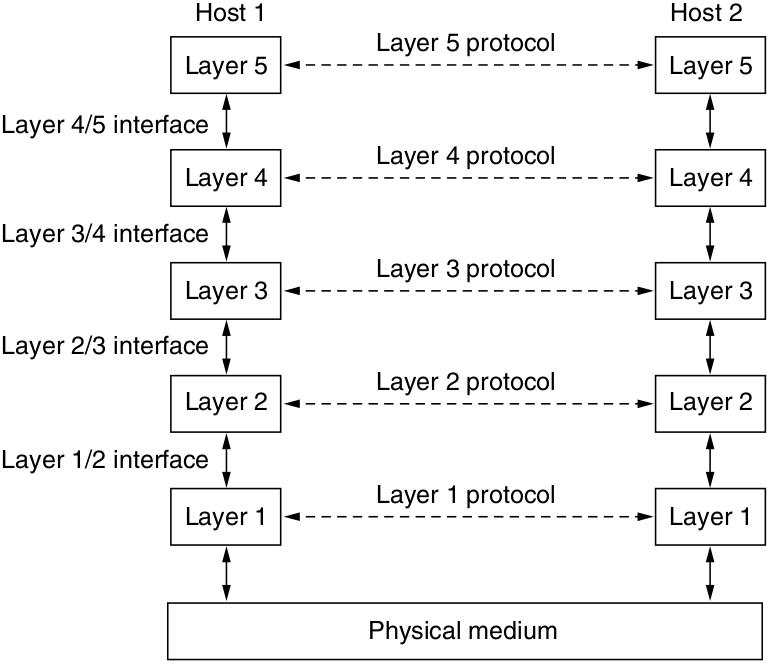
\includegraphics[width=0.7\textwidth]{figures/five_layer_network.png}
  \caption{Модел на пет слойна мрежа}
  \label{five_layer_network_fig}
\end{figure}

Между всяка съседна двойка слоеве има \textbf{интерфейс}. Този интерфейс
дефинира какви операции и услуги долният слой предлага на горния. Интерфейсите
между слоевете трябва да бъдат ясно дефинирани. Това впоследствие би улеснило
замяната на един слой с напълно различен протокол или имплементация (напр.
смяна на телефонни линии със сателитни такива), защото единственото, което се
очаква от новия протокол, е да предлага \textit{точно} същото множество услуги
на горния слой като стария. Аналогично, този механизъм позволява един протокол
да се промени в даден слой без знанието на слоевете под и над него.

\subsubsection{Основен механизъм на междуслойна комуникация. Капсулиране и
декапсулиране.}

Основния механизъм на междуслойна комуникация може да бъде описан с помощта на
пет слойния модел представен във \autoref{five_layer_network_fig}. Типично,
даден процес (т.е приложение) иска да изпрати съобщението \textit{M}. От петия
слой, съобщението бива предадено на четвъртия слой за трансмисия. Четвъртият
слой слага т.нар. \textbf{header} в началото на съобщението и предава резултата
към трети слой. Този header включва служебна информация, напр. адреси, за да
може съответния четвърти слой на приемната машина да достави съобщението. Други
примери за служебна информация могат да бъдат числови поредици (\textbf{sequence
numbers}), често използвани когато слоят на по-ниско ниво няма функционалност за
запазване на последователността на съобщенията, размери и времена.

\begin{figure}[h!]
  \centering
  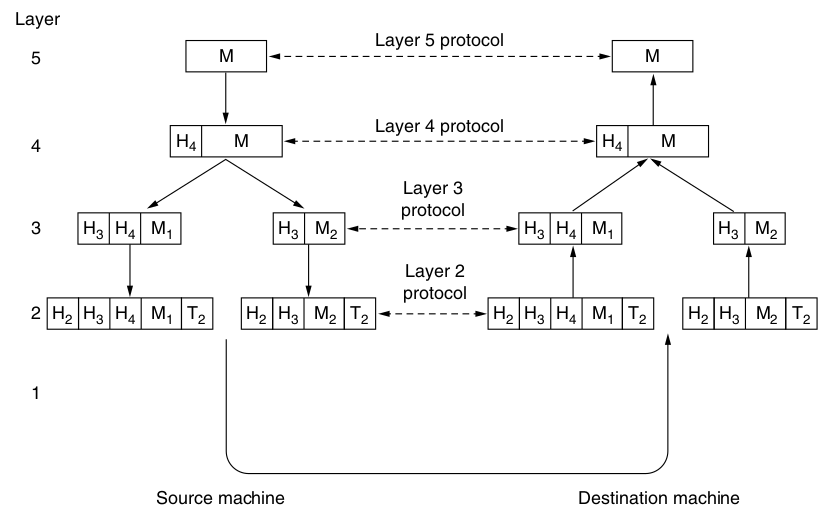
\includegraphics[width=1.0\textwidth]{figures/interlayer_communication.png}
  \caption{Междуслойна комуникация. Капсулиране и декапсулиране.}
  \label{interlayer_communication_fig}
\end{figure}

В много мрежи, често няма граница относно размера на съобщения на четвърти слой,
но почти винаги има такава относно размера от самият протокол на трети слой.
Следователно, третият слой трябва да раздели идващите съобщения на по-малки
единици --- пакети, като успоредно с това добавя header към всеки пакет. В
случая на \autoref{interlayer_communication_fig}, съобщението \textit{M} се
разделя на две части: M\textunderscript{1} и М\textunderscript{2}.

Третият слой аналогично предава пакетите на втория слой, който от своя страна
освен че добавя header, добавя и \textbf{опашка} (\textbf{trailer}). Резултата
се предава на първия слой, който се занимава с физическия пренос на данните.
Този процес е още известен като \textbf{капсулация} (\textbf{encapsulation}). В
приемащата страна, съобщението се декапсулира (\textbf{decapsulation}) като
всеки header се отделя успоредно с "изкачването" на съобщението нагоре по
слоевете. Нито един header за слоевете под \textit{n}-тия не достига до
\textit{n}-ти слой. Едновременно с това, на
\autoref{interlayer_communication_fig} ясно проличава виртуалната и реална
комуникация, както и разликите между протоколи и интерфейси. Например, на
четвърти слой процесите концептуално интерпретират комуникацията си като
хоризонтална използвайки протокола на четвърти слой и биха имали функции от типа
на send() и recieve(), въпреки че в реалност те комуникират със по-ниските
слоеве през 3/4 интерфейса, а не директно с другата страна.

\vfill

\section{Съществуващи решения и реализации}

\chapter{Проектиране на структурата на мрежов анализатор}

block diagrams?
\section{Функционални изисквания към мрежов анализатор}

what the analyzer should support

\section{Съображения за избор на програмни средства и развойна среда}

why c++ rocks, why angular rocks, show websocketpp benchmarks

\section{Проектиране на структурата на базата от данни}

??

explain orms / explain odb (if i integrate it) / show the db structure

\chapter{Програмна реализация на мрежов анализатор}

show sum code eh

\chapter{Ръководство на потребителя}

explaining how a sniffer works to noobs

\chapter{Заключение}

\begin{appendix}
\chapter{Изходен код}
\label{app_ex1}

%\section{Appendix}
%
%For many reasons some concept may be important for the document but too long for the main text. In this kind of cases these concept can be presented with the environment \imp{appendix} in appendices, e.g., as in \autoref{app_ex1} and \autoref{app_ex2}.

%%%%%%%%%%%%%%%%%%%%%%%%%%%%%%%%%%%%%%%%%%%%%%%%%%%%%%%%%%%
%%%%%%%%%%%%%%%%%%%%%%%%%%%%%%%%%%%%%%%%%%%%%%%%%%%%%%%%%%%

%\section{Footnotes}
%
%You may want to give additional information to some points\footnote{Bla bla} in the text\footnote{Blu blup}.

%\section{Index}
%
%If the document is very long, it may be very useful for a lot of readers to have an index for searching key words and certain concepts (Crtl+F is usually very helpful in PDFs but not always the best solution). For this, the  package \imp{makeidx}, the commands \imp{makeindex} and \imp{printindex} and the compiling option \imp{make index} are needed. You may want to index different words like heterogeneous materials\index{Heterogeneous materials}, effective properties\index{Effective properties} and homogenization\index{Homogenization}.


%\begin{appendix}

\end{appendix}

%\bibliographystyle{plain}
\bibliographystyle{abbrvnat}
\bibliography{literature/library}

\listoffigures
\listoftables

\printindex

\end{document}
